Pomocí metod založených na teorii funkcionálu hustoty (dále jen DFT metod) se v posledních zhruba dvaceti let provádí většina výpočtů elektronové struktury. Popularita DFT metod je dána jejich přijatelnou výpočetní náročností, která o mnoho nepřevyšuje náročnost Hartreeho-Fockovy 
metody. Výpočty jsou ale typicky daleko přesnější, neboť DFT metody zahrnují korelační energii. Efektivita DFT je dána tím, že nepracuje s poměrně složitou vlnovou funkcí (tj. funkcí 3$N$ souřadnic elektronů), ale s tzv. elektronovou hustotou, což je funkce pouze tří prostorových souřadnic. 
% (a k tomu jedné spinové souřadnice). 
V této kapitolce budeme používat stejnou notaci definovanou na začátku předchozí kapitoly.

Představme si základní pojmy. Začněme pojmem \textbf{funkcionál}. Pojďme si nejprve připomenout, jak funguje funkce. Do funkce vložíme nezávisle proměnou, tedy nějaké číslo, a na oplátku dostaneme číslo jiné, neboli závisle proměnnou. Jde tedy o zobrazení z prostoru čísel opět do prostoru čísel. U funkcionálu je to velmi podobné, akorát na vstupu není číslo, ale funkce. Pokud to tedy řekneme více matematicky, funkcionál je zobrazení z prostoru funkcí na prostor (kupř. reálných) čísel.

Takovým jednoduchým funkcionálem je například určitý integrál
$$
F[f(x)] = \int_a^b f(x) \mathrm{d}x.
$$
Určitý integrál potřebuje dodat vstupní funkci a po jeho vyčíslení dostaneme jedno jediné číslo. Povšimněte si zde zápisu funkcionálu pomocí hranatých závorek.  
Pro příklad funkcionálu v kvantové mechanice nemusíme chodit daleko, stačí se podívat na výraz pro energii
$$
E[\psi] = \int \psi^*\hat{H}\psi \mathrm{d}\tau .
\label{rov:dft:efunkc}
$$


Mezi funkcemi a funkcionály existují i další podobnosti. Pojmy jako minimum a maximum funkcionálu mají prakticky stejný význam. Existuje i funkcionální analogie k dobře známé derivaci funkce -- mluvíme o \textbf{variaci funkcionálu}.
Když provádíme derivování funkce, tak se vlastně díváme, co se děje se závisle proměnnou při malé změně nezávisle proměnné.
U variace je to podobné. Zajímá nás, jak se změní hodnota funkcionálu, když mírně změníme naši funkci. Přesná definice je složitější a neuvádíme ji zde. Bude ale pro nás důležité, že pro variace platí podobné vztahy, jako pro derivace. Dá se například ukázat, že v minimu funkcionálu je jeho variace nulová. Již dobře známý variační princip (konečně víme, proč se mu tak říká!) pak můžeme napsat jednoduše pomocí variace funkcionálu energie \eqref{rov:dft:efunkc} jako
\begin{equation}
\delta E[\Psi] = 0 .
\label{rov:dft:varprincip}
\end{equation}

Nyní se můžeme vrátit k definici ústřední veličiny této kapitoly -- elektronové hustoty $\rho(\mathbf{r})$.
Elektronová hustota má na rozdíl od vlnové funkce přímý fyzikální význam. Jedná se o pravděpodobnost, že v nějakém bodě prostoru najdeme \textbf{nějaký elektron}. Je důležité si uvědomit rozdíl mezi elektronovou hustotou a čtvercem vlnové funkce, který taktéž udává hustotu pravděpodobnosti. Čtverec vlnové funkce nám udává pravděpodobnost, že první elektron má spin $m_{s1}$ a nachází se v bodě $\mathbf{r}_1$, druhý elektron má spin $m_{s2}$ a nachází se v bodě $\mathbf{r}_2$ atd. Jedná se tedy o mnohem složitější veličinu, která závisí na celkem $4N$ proměnných ($N$ je počet elektronů), zatímco elektronová hustota závisí jen na třech proměnných.

Elektronová hustota souvisí s vlnovou funkcí systému dle vztahu
\begin{equation}
\rho=N \int |\psi(\textbf{r}_1,\textbf{r}_2,...,\textbf{r}_n)|^2 \mathrm{d}\textbf{r}_2\dots\mathrm{d}\textbf{r}_n .
\label{rov:dft:defrho}
\end{equation}
Integrujeme tedy čtverec vlnové funkce přes všechny elektrony kromě prvního. Zopakujme, že nás zajímá pravděpodobnost nalezení jakéhokoli elektronu, poloha ostatních nás nezajímá, a musíme tedy přes ně prointegrovat. První elektron ale není nijak odlišný od ostatních, stejně dobře bychom ale mohli udělat to samé pro druhý elektron. Jelikož je vlnová funkce antisymetrická, došli bychom ke stejnému výsledku. Z toho vyplývá násobící faktor $N$ před integrálem.
Z této definice hned plyne několik důležitých vlastností.

\begin{itemize}
\item Elektronová hustota je nezáporná veličina, platí tedy
\begin{equation}
\rho(\mathbf{r})  > 0 .
\end{equation}
\item Pokud zintegrujeme elektronovou hustotu přes celý prostor, dostaneme počet elektronů v systému jako
\begin{equation}
\int \rho\mathrm{d}r = N.
\end{equation}

\item V poloze jader má elektronová hustota maxima. Elektrony se totiž budou chtít pohybovat co nejblíže kladně nabitým jádrům (viz obrázek \ref{obr:dftvoda}). 

\item Pro tato maxima platí
%TOPETR: v poznamkach mas, ze to je nejaky teorem, ale neprectl jsem jaky....
\begin{equation}
\lim_{r_i \to 0} \left[ \frac{\delta}{\delta r}+2Z_A\right]\bar{\rho}(r)=0, 
\end{equation}
kde $\bar{\rho}$ je angulárně zprůměrovaná hodnota elektronové hustoty a $Z_A$ je náboj příslušného atomového jádra. Toto tvrzení není na první pohled zřejmé, ale nechť nám je čtenář pro teď věří.
\end{itemize}

\begin{figure}
\centering
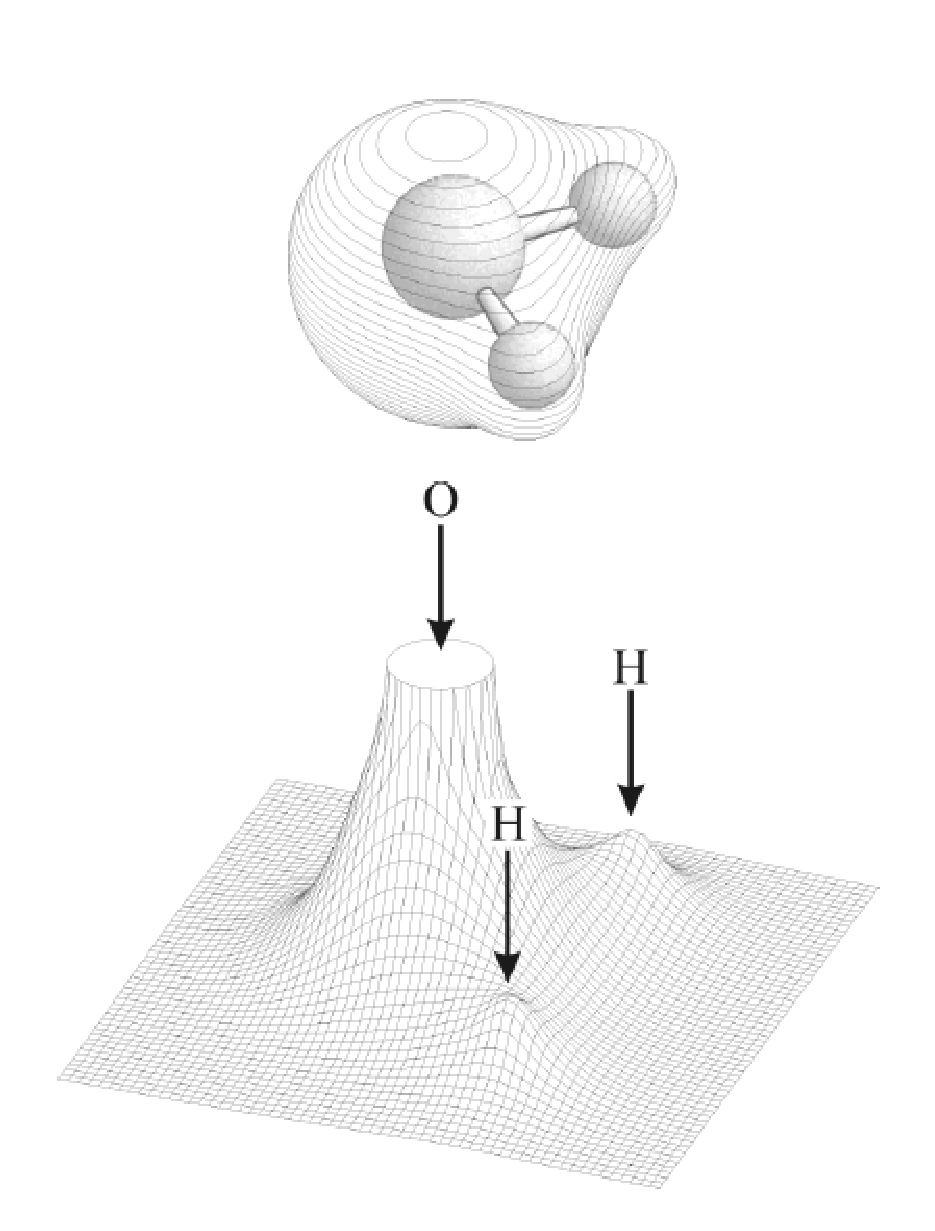
\includegraphics[scale=0.4]{DFTvoda.eps}
\caption[Elektronová hustota]{Tvar elektronové hustoty v molekule vody. (převzato z knihy \textit{A Chemist’s Guide to
Density Functional Theory, W. Koch a M. C. Holthausen,  Wiley-VCH})}
\label{obr:dftvoda}
\end{figure}

Z těchto vlastností vidíme, že pokud známe elektronovou hustotu, tak zároveň také můžeme zjistit počet elektronů, polohu jader i jejich náboj. To jsou ale přesně ty informace, které jsou potřeba ke specifikaci molekulárního hamiltoniánu
\begin{equation}
\hat{H}= -\frac{1}{2} \sum_{i=1}^N\Delta_i+\sum_{i=1}^N\sum_{j=i+1}^N\frac{1}{r_{ij}}-\sum_{i=1}^N\sum_{A=1}^K \frac{Z_A}{r_{iA}} ,
\label{rov:dft:molham}
\end{equation}
kde jsme vynechali pro jednoduchost člen popisující odpuzování jader, jenž je stejně v rámci Bornovy-Oppenheimerovy aproximace roven konstantě (použité symboly jsou vysvětleny na počátku kapitoly \ref{kap:abinitio}). Pokud ale elektronová hustota jednoznačně určuje hamiltonián, tak poté z řešení Schr\"odingerovy rovnice získáme taky energii a vlnovou funkci, a tudíž všechny potřebné veličiny. Podobným způsobem se zřejmě ubíraly úvahy Hohenberga a Kohna, kteří postavili teorii DFT na pevné fyzikální základy.

\subsection{Hohenbergovy-Kohnovy teorémy}

V roce 1964 publikovali Hohenberg s Kohnem slavný článek, který odstartoval vývoj DFT metod.
V tomto článku byly dokázány dva důležité teorémy. K jejich lepšímu pochopení si ještě musíme definovat pojem \textbf{externího potenciálu} $\nu_{ext}$, který nám říká, v jakém vnějším poli se elektrony pohybují. Externí potenciál má v případě hamiltoniánu \eqref{rov:dft:molham} tvar
\begin{equation}
\nu_{ext}=\sum_{i=1}^N\sum_{A=1}^K \frac{Z_A}{r_{iA}} ,
\end{equation} 
tj. jde o celkovou interakci elektronů s coulombickým potenciálem atomových jader. Jelikož se v DFT na vše díváme z pohledu elektronů, tak se tomuto potenciálu říká externí, protože nepochází ze samotných elektronů.
Je důležité si uvědomit, že externí potenciál vlastně definuje hamiltonián \eqref{rov:dft:molham}, neboť ostatní členy triviálně závisí pouze na počtu elektronů v systému. Molekula od molekuly či geometrie od jiné geometrie se liší právě externím potenciálem. Nyní již můžeme přejít ke slíbeným teorémům.

\textbf{První Hohenbergův-Kohnův teorém} hovoří o významnosti elektronové hustoty. Zní takto:

\bigskip
\noindent \uv{\textbf{Pro libovolný systém interagujících elektronů je externí potenciál $\nu_{ext}$ jednoznačně určen elektronovou hustotou} (až na konstantu)}

\bigskip
Důsledek tohoto tvrzení jsme si již naznačili dříve. Pokud máme jednoznačně daný externí potenciál, pak také známe hamiltonián a můžeme v principu spočítat vlnovou funkci i energii, které jsou tudíž jednoznačně určeny pouze elektronovou hustotou. \textbf{Elektronová energie je tedy jednoznačným funkcionálem elektronové hustoty} neboli v matematickém zápisu
\begin{equation}
E_{el}=E_{el}[\rho] .
\end{equation}
Pokud bychom tedy tento funkcionál znali a znali také správnou hustotu, tak bychom mohli získat energii i bez řešení Sch\"{o}dingerovy rovnice a hledání vlnových funkcí.
Dokažme si nyní toto tvrzení. 

\textbf{Pomocné tvrzení}: Nejprve si musíme odvodit pomocný vztah pro střední hodnotu externího potenciálu.
Rozepišme si nejprve externí potenciál na součet jednoelektronových příspěvků:
\begin{equation}
\nu_{ext}=\sum_{i=1}^N \nu_i = \sum_{i=1}^N \sum_{A=1}^K \frac{Z_A}{r_{iA}}.  
\label{rov:dft:nui}
\end{equation}
Pojďme si nyní vyčíslit integrál
\begin{equation}
\int \nu_{ext} \psi(\textbf{r}_1,...,\textbf{r}_N)^2\mathrm{d}\tau .
\end{equation}
Dosazením vztahu \eqref{rov:dft:nui} a vhodným přeuspořádáním mnohonásobného integrálu dostaneme
\begin{equation}
\sum_i^N \int \nu_i \left[\int \psi(\mathbf{r}_1,...,\mathbf{r}_N)\prod_{j\neq i}\mathrm{d}\textbf{r}_j\right] \mathrm{d}\textbf{r}_i .
\end{equation}
Výraz v hranaté závorce není ale nic jiného než elektronová hustota $\rho$ (až na násobný faktor $N$), dostáváme tedy finální vztah
\begin{equation}
\int \nu_{ext} \psi(\textbf{r}_1,...,\textbf{r}_N)^2\mathrm{d}\tau = \sum_{i=1}^N \int \nu_i(\textbf{r}_i)\frac{\rho(\textbf{r}_i)}{N}\mathrm{d}\mathbf{r}_i= \int \nu(\textbf{r})\rho(\textbf{r}) \mathrm{d}\mathbf{r} ,
\label{rov:dft:intnupsi}
\end{equation}
neboť potenciál $\nu_i$, ve kterém se pohybuje $i$-tý elektron, je pro každý elektron identický.

\bigskip 
\textbf{Důkaz HK1:} Důkaz se provádí sporem. Předpokládejme, že jedné dané hustotě $\rho$ přísluší dva různé externí potenciály $\nu_{ext1}$ a $\nu_{ext2}$, kterým přísluší hamiltoniány $\hat{H}_1$ a $\hat{H}_2$ a vlnové funkce $\psi_1$ a $\psi_2$.  Pak díky variačnímu principu musí platit

\begin{equation}
E_1 = \int \psi_1^* \hat{H}_1 \psi_1 \mathrm{d}\tau < \int \psi_2^* \hat{H}_1 \psi_2 \mathrm{d}\tau ,
\end{equation}
protože když ve funkcionálu energie k hamiltoniánu $\hat{H_1}$ přiřadíme funkci $\psi_2$, která není jeho vlastní funkcí základního stavu, tak musíme dostat větší energii než při použití skutečné vlastní funkce $\psi_1$. Nyní mazaně přepíšeme pravou stranu nerovnosti jako  
\begin{equation}
\int \psi_2^* \hat{H}_1 \psi_2 \mathrm{d}\tau = \int \psi_2^* \hat{H}_2 \psi_2\mathrm{d}\tau  + \int \psi_2^* \left[\hat{H}_1-\hat{H}_2\right] \psi_2\mathrm{d}\tau = E_2 + \int \rho(\mathbf{r})(\nu_1-\nu_2)\mathrm{d}\mathbf{r}.
\end{equation}
V poslední rovnosti jsme využili toho, že oba hamiltoniány se liší pouze externím potenciálem, a použili jsme vztah \eqref{rov:dft:intnupsi}.

\noindent Vyšlo nám tedy, že platí nerovnost
\begin{equation}
E_1 < E_2+\int \rho(\mathbf{r})(\nu_1-\nu_2)\mathrm{d}\mathbf{r}.
\label{rov:HK1_1}
\end{equation}
Tu samou argumentaci bychom ale mohli také aplikovat opačně a dostali bychom
\begin{equation}
E_2 < E_1+\int \rho(\mathbf{r})(\nu_2-\nu_1)\mathrm{d}\mathbf{r} .
\label{rov:HK1_2}
\end{equation}
Sečtením obou rovnic \eqref{rov:HK1_1} a \eqref{rov:HK1_2} tedy dostáváme
\begin{equation}
E_1 + E_2 < E_2 + E_1 ,
\end{equation}
což nemůže platit, a tedy náš původní předpoklad o existenci dvou různých externích potenciálů je také chybný.
\hfill {\footnotesize $\blacksquare$}

\bigskip
Formálně můžeme funkcionál energie napsat jako
\begin{equation}
E=\int \psi^*\hat{H}\psi \mathrm{d}\tau = \int \psi^*\hat{T}\psi\mathrm{d}\tau + \int \psi^*\hat{V_{el}}\psi\mathrm{d}\tau + \int \psi^*\nu_{ext}\psi\mathrm{d}\tau=\hat{T}[\rho]+\hat{V}_{ee}[\rho]+\hat{V}_{ne}[\rho] .
\end{equation}
Vidíme, že funkcionál energie se stejně jako příslušný hamiltonián \eqref{rov:dft:molham} skládá ze tří různých příspěvků: funkcionálu kinetické energie elektronů $\hat{T}[\rho]$, funkcionálu repulze elektronů $\hat{V}_{ee}[\rho]$ a funkcionálu interakce elektronů s jádry (obecně s externím potenciálem) $\hat{V}_{ne}[\rho]$. 
Explicitní tvar posledně jmenovaného funkcionálu jsme si již vlastně odvodili rovnicí \eqref{rov:dft:intnupsi} a platí tedy
\begin{equation}
\hat{V}_{ne}[\rho] = \int \nu_i(\textbf{r})\rho(\textbf{r}) \mathrm{d}r .
\end{equation}
Součet zbylých dvou funkcionálů nazýváme Hohenbergovým-Kohnovým funkcionálem a značíme $F_{HK}[\rho]$. 
Celkový funkcionál energie tedy můžeme zapsat jako
\begin{equation}
E[\rho] = \hat{T}[\rho]+\hat{V}_{ee}[\rho]+\hat{V}_{ne}[\rho] = F_{HK}[\rho] + \int \nu_i(\mathbf{r})\rho(\textbf{r}) \mathrm{d}r .
\end{equation}

Přesný tvar Hohenbergova-Kohnova funkcionálu $F_{HK}[\rho]$ bohužel není dodnes znám. 
Ovšem i kdybychom jej znali, tak nám stále něco schází k jeho úspěšného použití. Nevíme totiž, jak získat pro daný systém správnou elektronovou hustotu $\rho$, kterou bychom do něj mohli dosadit. Samozřejmě kdybychom znali vlnovou funkci, tak stačí dosadit do definičního vztahu \eqref{rov:dft:defrho}. Tomu se ale právě chceme vyhnout! Smyslem celé teorie funkcionálu hustoty je vyhnout se přímému řešení elektronové Schr\"{o}dingerovy rovnice.

Cestu k elektronové hustotě nám dává druhý teorém od Hohenberga a Kohna, který zní takto:

\bigskip
\textbf{Předpokládejme, že danému externímu potenciálu $\nu_{ext}$ přísluší elektronová hustota $\rho_0$. Pak pro jakoukoli jinou elektronovou hustotu\footnote{Přesněji řečeno, daná elektronová hustota musí být takzvaně $\nu$-{reprezentovatelná}, neboli musí k ní příslušet nějaký externí potenciál. Pro funkce, které toto nesplňují, 2. HK teorém neplatí.} $\rho^{\prime}$ bude platit:}
\begin{equation}
E[\rho_0] < E[\rho^{\prime}] .
\label{rov:dft:HK2}
\end{equation}

Nejedná se o nic jiného než variantu variačního principu, který taky využijeme k důkazu.

\bigskip
\textbf{Důkaz:} Z prvního HK teorému plyne, že jakákoli funkce $\rho^{\prime}$ patří k externímu potenciálu $\nu_{ext}^{\prime}$, který je odlišný od $v_{ext}$, a přísluší k němu vlnová funkce $\psi^{\prime}$. Pokud ale pro tuto vlnovou funkci vyčíslíme energii, pak nám z již známého variačního principu plyne
\begin{equation}
\int \psi^{\prime *} \hat{H} \psi^{\prime} \mathrm{d}\tau = E[\rho] > E [\rho_0],
\end{equation}
což jsme chtěli dokázat. \hfill {\footnotesize $\blacksquare$}

Druhý HK teorém nám tedy dává principiální návod, jak hledat elektronovou hustotu. Budeme hledat přes všechny možné hustoty a správná bude ta, která nám dá nejnižší energii.

Hohenbergovy-Kohnovy teorémy dávají DFT solidní fyzikální základ, moc nás ale neposunují k praktické aplikaci, jelikož neznáme přesný funkcionál $F_{HK}[\rho]$.
Praktickou cestu k DFT výpočtům ukázali až o rok později Kohn s Shamem.

\subsection{Kohnovy-Shamovy rovnice}

Nyní stojíme před zásadním problémem nalezení alespoň přibližného funkcionálu $F_{HK}[\rho]$, ve kterém je zahrnuta kinetická energie elektronů, klasická coulombická interakce mezi elektrony a dále korelační a výměnné efekty. 
%Obecně bychom chtěli spočítat co největší část energie pomocí známých dobře definovaných přibližných vztahů a zbylé části poté můžeme modelovat a odchylky poté můžeme modelovat třeba semiempiricky.(\footnote{Tento přístup by se dal přirovnat k situaci v chemické termodynamice, ve které počítáme se vzorečky platnými pro ideální chování a odchylky schováváme do aktivitních koeficientů).
Ukázalo se, že největší potíže činí dostatečně přesné vyjádření funkcionálu pro kinetickou energii.
Tento problém je tak zásadní, že budeme muset částečně obětovat náš původní cíl a vrátit se k molekulovým orbitalům popisujícím nezávislý pohyb elektronů.
Pokud totiž máme $N$ elektronů, kde $i$-tý elektron je umístěn v molekulovém orbitalu $\varphi_i$, můžeme vyčíslit kinetickou energii dle vztahu
\begin{equation}
E_{kin}=-\frac{1}{2}\sum_{i=1}^N \int \varphi \Delta_i \varphi \mathrm{d}\textbf{r}_i .
\end{equation}
Tj. spočítáme kinetickou energii pro každý elektron popsaný jednoelektronovou vlnovou funkcí (orbitalem) a energie sečteme. S takto postavenou teorií přišli v roce 1965 Kohn s Shamem.

\hyphenation{me-zi-elektron-ové}
Obecná strategie odvození Kohnovy-Shamovy procedury je následující. Definuje se fiktivní systém neinteragujících elektronů (podobně jako v Hartreeho-Fockově teorii zde elektrony interagují pouze skrze efektivní potenciál), který je zvolen tak, aby jeho elektronová hustota byla rovna elektronové hustotě reálného systému. 
Funkcionál energie se rozepíše následujícím způsobem:
\begin{equation}
E[\rho]= T_{n}[\rho] + \frac{1}{2}\int \int \frac{\rho(\textbf{r}_1)\rho(\textbf{r}_2)}{r_{12}}\mathrm{d}\textbf{r}_1\mathrm{d}\textbf{r}_2 + V_{nekl}(\rho) +\left\lbrace T[\rho]-T_{n}[\rho]\right\rbrace + \int \nu \rho \mathrm{d}\textbf{r},
\label{rov:dft:KSfunkc}
\end{equation}
kde $T_{n}[\rho]$ je kinetická energie neinteragujícího systému, druhý člen odpovídá klasické mezielektronové repulzi (násobí se jednou polovinou, aby se interakce nezapočítávaly dvakrát), $V_{nekl}$ zahrnuje korelační a výměnnou energii elektronů, člen ve složené závorce je rozdíl kinetických energií reálného a neinteragujícího systému  a poslední člen odpovídá interakci elektronů s jádry. Pokud všechny neznámé členy dáme dohromady, dostaneme tzv. korelačně-výměnný potenciál
\begin{equation}	
E_{XC}[\rho]=\left[T[\rho]-T_{n}[\rho]\right] +  V_{nekl} .
\label{rov:dft:exc}
\end{equation}
% V_{ee}(\rho) - \frac{1}{2}\int \int \frac{\rho(\textbf{r}_1)\rho}{\textbf{r_{12}}}
Pokud na funkcionál \eqref{rov:dft:KSfunkc} nyní aplikujeme variační princip, tak dostaneme rovnice, které mají stejný tvar jako rovnice
pro systém neinteragujících elektronů. Jenže pro tento systém známe řešení! Stačí vyřešit příslušnou jednoelektronovou Schr\"{o}dingerovu rovnici
\begin{equation}
\left(-\frac{1}{2}\Delta_i + V_{eff} \right) \varphi_i =\epsilon_i \varphi_i ,
\label{rov:dft:KSeq}
\end{equation}
kde $V_{eff}$ je efektivní potenciál, pro který platí
\begin{equation}
V_{eff}=\nu_{ext}+\frac{1}{2}\frac{\rho(\textbf{r}^{\prime})}{|\textbf{r}-\textbf{r}^{\prime}|}\mathrm{d}\textbf{r}^{\prime}+u_{xc} ,
\end{equation}
kde $u_{xc}$ je funkcionální derivace (variace) výměnně-korelačního funkcionálu \ref{rov:dft:exc}.\footnote{V našem odvození postupujeme dosti svižně. Pro případného zájemce o podrobnější pohled na DFT doporučujeme klasickou publikaci R. G. Parr, W. Yang \textit{Density-Functional Theory of Atoms and Molecules.} Oxford University Press, 1989} Tvar tohoto potenciálu byl odvozen tak, aby byly elektronové hustoty reálného i fiktivního systému stejné.
Rovnice \ref{rov:dft:KSeq} se nazývají Kohnovy-Shamovy a řeší se podobně jako rovnice Hartreeho-Fockovy rozvojem do báze AO.
Získáme tak sadu molekulových orbitalů, ze kterých pak dostaneme elektronovou hustotu dle vztahu (uvádíme bez důkazu)
\begin{equation}
\rho(\textbf{r}) = \sum_{i=1}^N |\varphi|_i^2.
\label{rov:dft:KSrho}
\end{equation}
%Jelikož neinteragující systém byl definován tak, aby 
Tuto hustotu pak můžeme dosadit do funkcionálu \eqref{rov:dft:KSfunkc} a získáme tak požadovanou energii.

Kohnův-Shamův přístup je v principu přesný, pokud bychom znali přesný tvar výměnně-korelačního funkcionálu $E_{XC}[\rho]$.
Ten sice neznáme, ale existuje spousta vztahů přibližných, o kterých pojednávají další kapitoly.

\subsection{Teorie funkcionálu hustoty v kvantové chemii}

Problém, který KS metoda přímo neřeší, je nalezení tvaru výměnně-korelačního potenciálu.
V zásadě existují dva přístupy k tomuto problému. V prvním přístupu se snažíme odvodit vhodný funkcionál $E_{xc}$ čistě pomocí teoretických argumentů z pokročilejších partií DFT. Druhý přístup je pragmatičtější. Konkrétní tvar funkcionálu může obsahovat parametry, které se určují z experimentálních dat. V praxi se oba tyto přístupy často kombinují.

Existuje několik různých rodin funkcionálů, které se liší mírou přesnosti, výpočetními nároky i svým zaměřením, a které jsou podrobněji rozebrány v následujících podkapitolách.

\subsubsection{Aproximace lokální hustoty}

Aproximace lokální hustoty (angl. \textit{Local Density Approximation}, LDA) vychází z tzv. modelu \textbf{homogenního elektronového plynu} (HEG). Je to hypotetický fyzikální stav, kdy máme všude konstantní elektronovou hustotu, vyváženou rovnoměrným pozitivním pozadím. Tento model je pro teorii DFT velmi užitečný, neboť pro něj existují přesné výpočty a simulace. Tento model byl ale kdysi užitečný i pro chemiky, dají se takto třeba popsat valenční elektrony v kovech (teorie elektronového plynu). Jak ale tento model použít na atomy nebo molekuly, které mají elektronovou hustotu značně nehomogenní (elektronová hustota je velká v oblasti jader a pak postupně pravděpodobnost nalezení elektronů klesá)?

Můžeme si představit, že prostor okolo atomu/molekuly rozdělíme na malinké krychličky. Ve středu každé krychličky zjistíme elektronovou hustotu, kterou poté dosadíme do vztahů plynoucích z teorie HEG.
Získáme tím elektronovou energii v této malé krychličce a celkovou energii získáme součtem přes všechny krychličky. Matematicky rigorózně to můžeme zapsat pomocí trojného integrálu přes celý prostor
\begin{equation}
E_{XC}^{LDA}[\rho]=\int \rho(\textbf{r}) \varepsilon(\rho(\textbf{r})) \mathrm{d}\textbf{r} ,
\end{equation}
kde $\varepsilon(\rho(\textbf{r}))$ je výměnně-korelační energie HEG o hustotě $\rho$ vztažená na jeden elektron. Tato rovnice definuje výše zmíněnou aproximaci lokální hustoty.

Jaký je konkrétní tvar $\varepsilon(\rho(\textbf{r}))$? Nejprve jej rozdělíme na korelační a výměnnou část (takto to dělá většina DFT metod)
\begin{equation}
\varepsilon(\rho(\textbf{r}))=\varepsilon_x(\rho)+\varepsilon_c(\rho) .
\end{equation}

\noindent Pro výměnnou část se dá odvodit následující analytický vztah
\begin{equation}
V_x[\rho]=-\frac{3}{4}\left(\frac{3}{\pi}\right)^{\frac{1}{3}}\rho^{\frac{1}{3}}.
\end{equation}
Tento vztah je spojen s jménem Slater\footnote{Ano, je ten ten samý pan Slater, podle kterého jsou pojmenované naše oblíbené determinanty.}, označuje se tedy zkratkou S.

Pro korelační energii HEG nelze získat analytický výraz. Příslušné výpočty lze ale provést numericky a výsledek poté nafitovat. Výsledný korelační funkcionál je znám jako VWN (dle pánů Voska, Wilka a Nusaira). V kombinaci se Slaterovým výrazem pro výměnnou část získáme metodu SVWN (výměnná část se ve zkratce uvádí vždy první).

Mírným vylepšením je metoda spinově závislé aproximace lokální hustoty (angl. \textit{Local Spin Density Approximation}, LSDA), které pracují zvlášť s elektronovou hustotou elektronů se spinem $\alpha$ a zvlášť se spinem $\beta$.

Metoda LDA byla prvním větším úspěchem DFT teorie. Její výsledky jsou typicky o něco lepší než metoda Hartreeho-Focka a můžeme ji s úspěchem použít pro stanovení geometrií, vibračních frekvencí nebo dipólových momentů. Na druhou stranu funguje méně dobře pro energetiku chemických reakcí. Dnes se metoda LDA používá zřídka, nahradily ji pokročilejší metody.

\subsubsection{GGA funkcionály}
Jednou z nevýhod DFT je absence jasné cesty k přesnějším výsledkům, neboť neznáme tvar výměnně-korelačního členu. U \textit{ab initio} metod naproti tomu jasně víme, jak alespoň v principu dospět k přesnému výsledku (např. metodou Full CI ve velké bázi).

Jednou z možností postupu, která se nám po předchozí kapitole nabízí, je zkusit vyjít z aproximace lokální hustoty a tu se snažit dále vylepšit. V LDA jsme v daném bodě využívali pouze hodnotu elektronové hustoty. Taylorův rozvoj nám napovídá, že by mohlo být užitečné využít informaci o \textbf{gradientu hustoty} $\nabla\rho(\textbf{r})$. 
Tím se dostaneme k metodám \textbf{zobecněného gradientu} (z angl. \textit{Generalized Gradient Approximation}, GGA), pro které má výměnně-korelační funkcionál obecný tvar
\begin{equation}
E_{xc}^{GGA}=\int \rho(\textbf{r})f(\rho,\nabla\rho) \mathrm{d}\textbf{r} .
\end{equation}
Konkrétní tvar těchto funkcionálů již bývá značně složitý a často obsahuje nastavitelné parametry. Mezi nejznámější výměnné GGA funkcionály patří například Beckeho výměnný funkcionál (zkratka \textbf{B88}, nebo jen B), který obsahuje jeden parametr. Mezi známé korelační funkcionály patří například \textbf{LYP} (od pánů Lee, Yang a Paara) nebo \textbf{P86} (autor Perdew). Jejich kombinací pak získáme často užívané metody \textbf{BP86} a \textbf{BLYP}. Dalším výměnně-korelačním funkcionálem je \textbf{PBE} (Perdew, Burke, Erzenhof) z roku 1996, který neobsahuje žádné parametry.

GGA funkcionály jsou značně přesnější než LDA, a proto právě tyto funkcionály odstartovaly masové používání DFT v kvantové chemii.

Dalším logickým krokem ke zlepšení je využití dalších informací kromě gradientu, například druhé derivace. Mluvíme potom o \textbf{meta-GGA funkcionálech}, mezi které patří například korelační funkcionál B95 nebo výměnně-korelační funkcionál TPSS.

\subsection{Hybridní funkcionály}
Pozorný čtenář by se mohl ptát, proč vlastně k výpočtu výměnné energie nevyužijeme Kohn-Shamovy orbitaly, když je konec konců používáme pro výpočet kinetické energie. Využili bychom vzoreček známý z HF teorie 
\begin{equation}
E_X^{exact}=-\frac{1}{2}\sum_{i=1}^N\sum_{j=1}^N K_{ij} . 
\label{rov:dft:exHF}
\end{equation}
Bohužel se ukázalo, že přímé použití tohoto vzorce (spolu s nějakým korelačním funkcionálem) nevede k dobrým výsledkům, jelikož se tím naruší kompenzace chyb v současných funkcionálech.

Zlepšení ovšem dosáhneme, pokud oba přístupy zkombinujeme a část výměnné energie vypočítáme přesně ze vzorce \ref{rov:dft:exHF} a zbylou část pomocí dříve zmíněných výměnných funkcionálů. Tím dostaneme takzvané hybridní funkcionály, které představují další výrazné zlepšení přesnosti.
Mezi hybridní funkcionály patří i funkcionál \textbf{B3LYP}, který je v současnosti suverénně nejpoužívanější kvantově-chemickou metodou (přestože byl vyvinut už v roce 1993).
Jeho přesný tvar je
\begin{equation}
E_{xc}^{B3LYP}=(1-a_0-a_x)E_x^{LDA}+a_0E_x^{exact}+a_xE_x^{B88}+(1-a_c)E_c^{VWN}+a_c E_c^{LYP}
\end{equation}
a nastavitelné parametry mají hodnotu $a_0=0{,}2$, $a_x=0{,}72$ a $a_c=0{,}81$.
Parametr $a_0$ určuje procento přesné výměnné energie; B3LYP má tedy 20\% podíl HF výměnné energie.

Z dalších mnoha hybridních funkcionálů uveďme alespoň (v závorkách uvádíme procento HF výměnné energie): PBE0 (25\,\%), BMK (50\,\%), BHandHLYP(50\,\%)

\subsubsection{Moderní funkcionály}
Oblast DFT metod patří díky její užitečnosti ke stále velmi aktivním oblastem výzkumu v kvantové chemii. V současnosti už existují stovky různých funkcionálů. V posledních letech se objevilo mnoho různých nových typů kromě výše zmíněných. Za zmínku stojí kupříkladu tzv. \textbf{dvojitě hybridní funkcionály}. Ty v sobě kombinují metodu DFT s poruchovou metodou. V prvním kroku vypočítáme Kohnovy-Shamovy orbitaly pomocí hybridního funkcionálu

\begin{equation}
E_{xc}^{hybrid}=a_1E_x^{GGA}+(1-a_1)E_x^{EXACT}+a_2E_c^{GGA},
\end{equation}

v kroku druhém pak zformulujeme vylepšený funkcionál

\begin{equation}
E_{xc}^{DH}=E_{xc}^{hybrid}+(1-a_2)E_c^{KS-MP2},
\end{equation}

kde $E_c^{KS-MP2}$ je vypočítáno jako MP2 korekce energie s použitím Kohnových-Shamových orbitalů. S tímto výměnně-korelačním členem pak vypočítáme energii molekuly. Nastavitelné parametry jsou kupříkladu pro metodu B2LYP zvoleny takto: $a_1=0,47$, $a_2$=0,73.
Výsledky získané touto metodou jsou poměrně kvalitní, ale na druhou stranu je tato metoda výpočetně také značně náročná.

Viděli jsme také, že s kvalitou výsledku dokáže hodně pohnout přídavek výměnného členu toho typu, který nacházíme v HF metodě. V hybridních funkcionálech tento člen přidáváme pro všechny mezi-elektronové vzdálenosti. Jinou možností je použít lokální funkcionály pro malé mezi-elektronové vzdálenosti a HF výměnný člen pro velké mezi-elektronové vzdálenosti. Mluvíme pak o tzv. \textbf{range-separated funkcionálech}. Ty jsou užitečné například při výpočtech excitovaných stavů. 
%Mělo by platit, že $lim_{V_x\to \infty}=\frac{1}{r}$
%zmínka o self-interakční chybě.

Jedním ze slabých míst DFT je omezená schopnost této teorie popsat tzv. disperzní interakci (více viz kapitola \ref{kap:mezimolsily}).
Existují různě složité cesty k nápravě. Vůbec nejjednodušší metodou je použít funkcionál, ve kterém disperzní příspěvek vůbec přítomen není, a tento příspěvek pak modelovat empiricky (\textit{Dispersion-corrected functional}).  

%Grimmeho empirická korekce
%\begin{equation}
%E_{vdw}=-s_6\sum c^{ij}r_{ij}^{-6}
%\end{equation}
%Koeficient $s_6$ závisí na použitém funkcionálu, zatímco koeficienty $c_{ij}$ závisí na typu interagujících atomů.

I přes své stáří však pro rutinní výpočty stále dominuje funkcionál B3LYP díky jeho velké univerzalitě a přesnosti.
Pro detailní přehled starších i moderních funkcionálů lze nahlédnout do návodu k programu Gaussian\footnote{\url{http://www.gaussian.com/g\_tech/g\_ur/k\_dft.htm}}.

%\textbf{Jakobův žebřík, obrázek (Genesis 28:10-12)}
